%% Glaukopis -- International Journal of Information Security (Springer) submission, v1.6-ijis (2026-10-24).
%% Port of doc/v1.6/glaukopis_v1.6.tex to Springer's svjour3 class in the journal's required
%% "twocolumn" format, numbered references (spmpsci.bst), single-blind (author-identified).
%% Build: bash build.sh   (pdflatex -> bibtex -> pdflatex x2); needs svjour3.cls, svglov3.clo, spmpsci.bst (in this folder).
%% Review model is single-blind (journal guidelines), so author names and affiliations stay in the manuscript.

\documentclass[border=3pt]{standalone}

\usepackage[T1]{fontenc}
\usepackage{amsmath,amssymb}
\usepackage{booktabs,array,tabularx,multirow}
\usepackage{graphicx}
\usepackage{xcolor}
\usepackage{xurl}
\usepackage{tikz}
\usetikzlibrary{arrows.meta,positioning,fit,backgrounds,calc}
\usepackage{pgfplots}
\usepgfplotslibrary{groupplots}
\pgfplotsset{compat=1.15}
\usepackage{listings}

\setlength{\emergencystretch}{2em}
\renewcommand{\topfraction}{0.95}
\renewcommand{\bottomfraction}{0.95}
\renewcommand{\textfraction}{0.03}
\renewcommand{\floatpagefraction}{0.75}
\setcounter{topnumber}{4}\setcounter{bottomnumber}{4}\setcounter{totalnumber}{8}\setcounter{dbltopnumber}{4}
\lstset{basicstyle=\footnotesize\ttfamily,breaklines=true,columns=fullflexible,keepspaces=true,frame=single,showstringspaces=false}
\newcommand{\code}[1]{\path{#1}}
\newsavebox{\fitbox}
\newcommand{\fitwidth}[1]{\sbox{\fitbox}{#1}\ifdim\wd\fitbox>\textwidth\resizebox{\textwidth}{!}{\usebox{\fitbox}}\else\usebox{\fitbox}\fi}
\newcommand{\ci}[2]{{\scriptsize[#1,\,#2]}}
\newcommand{\Abal}{A_{\mathrm{bal}}}
\newcommand{\Bbal}{B_{\mathrm{bal}}}
\newcommand{\Tbal}{T_{\mathrm{bal}}}
\definecolor{seriesblue}{HTML}{2A78D6}
\definecolor{refgray}{HTML}{52514E}


\begin{document}\setlength{\textwidth}{174mm}

\resizebox{\textwidth}{!}{%
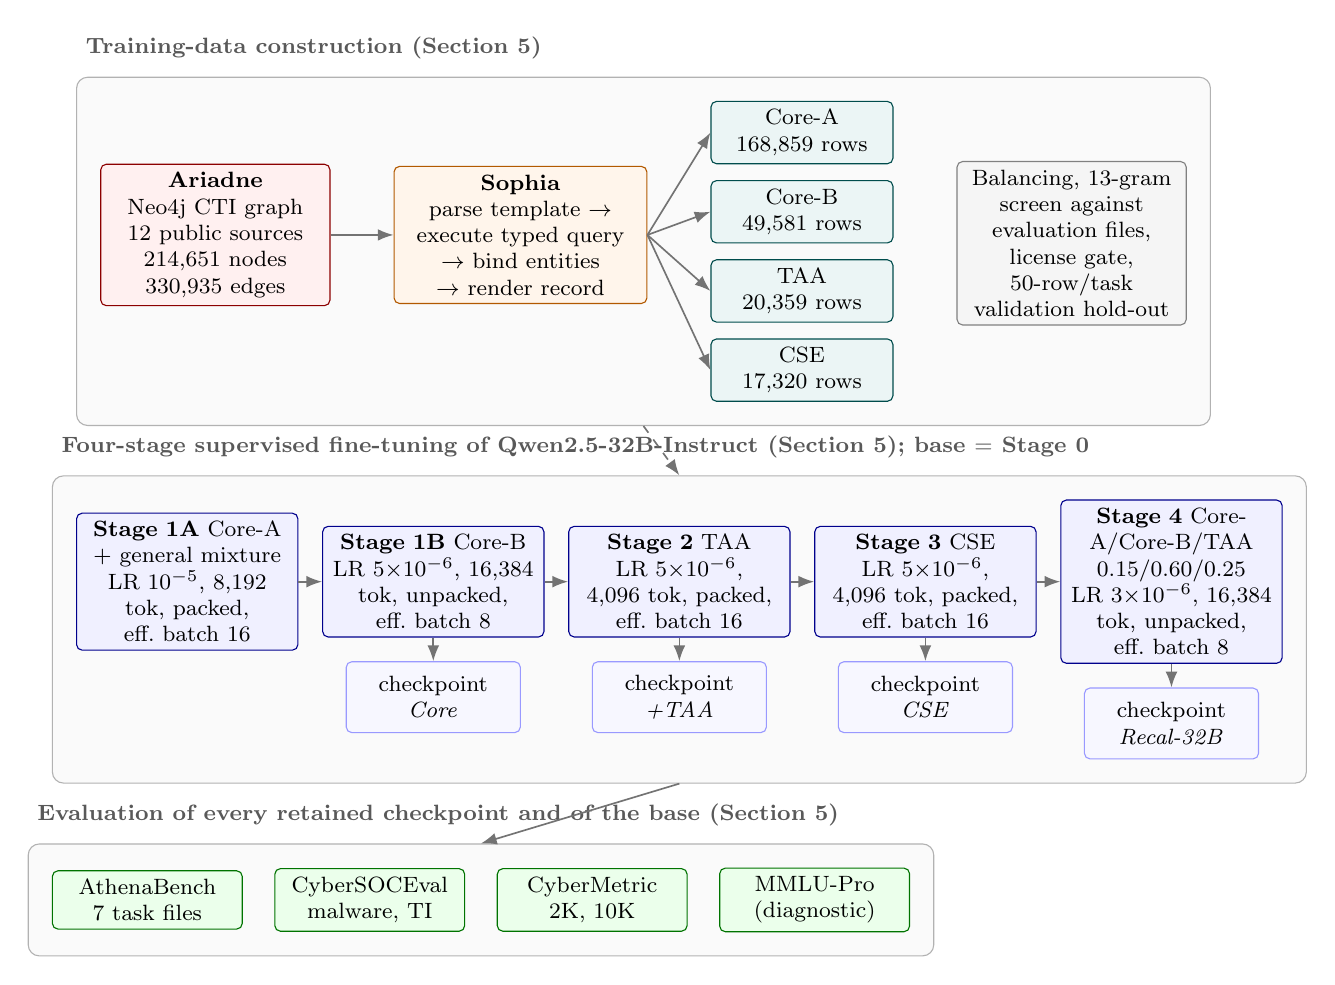
\begin{tikzpicture}[
  font=\footnotesize, >={Latex[length=2mm]}, node distance=3mm and 4mm,
  box/.style={draw, rounded corners=2pt, align=center, inner sep=3pt, minimum height=9mm},
  src/.style={box, fill=red!6, draw=red!55!black, text width=27mm},
  gen/.style={box, fill=orange!8, draw=orange!70!black, text width=30mm},
  shard/.style={box, fill=teal!8, draw=teal!60!black, text width=21mm, minimum height=7mm},
  stage/.style={box, fill=blue!6, draw=blue!55!black, text width=26mm},
  ev/.style={box, fill=green!8, draw=green!45!black, text width=22mm, minimum height=7mm},
  arr/.style={->, semithick, black!55}, grp/.style={draw=black!30, rounded corners=4pt, inner sep=3mm, fill=black!2},
  lbl/.style={font=\footnotesize\bfseries, text=black!65}]
\node[src] (ari) {\textbf{Ariadne}\\Neo4j CTI graph\\12 public sources\\214,651 nodes\\330,935 edges};
\node[gen, right=8mm of ari] (sop) {\textbf{Sophia}\\parse template $\to$ execute typed query $\to$ bind entities $\to$ render record};
\node[shard, right=8mm of sop, yshift=13mm] (sa) {Core-A\\168,859 rows};
\node[shard, below=2mm of sa] (sb) {Core-B\\49,581 rows};
\node[shard, below=2mm of sb] (st) {TAA\\20,359 rows};
\node[shard, below=2mm of st] (sc) {CSE\\17,320 rows};
\node[box, fill=black!4, draw=black!50, text width=27mm, right=8mm of sb, yshift=-4mm] (scr) {Balancing, 13-gram screen against evaluation files, license gate, 50-row/task validation hold-out};
\draw[arr] (ari) -- (sop);
\foreach \s in {sa,sb,st,sc} \draw[arr] (sop.east) -- (\s.west);
\begin{scope}[on background layer]
 \node[grp, fit=(ari)(sop)(sa)(sc)(scr)] (g1) {};
\end{scope}
\node[lbl, above=1mm of g1.north west, anchor=south west] {Training-data construction (Section 5)};
% stages
\node[stage, below=11mm of g1.south west, anchor=north west] (s1) {\textbf{Stage 1A} Core-A + general mixture\\LR $10^{-5}$, 8,192 tok, packed, eff.\ batch 16};
\node[stage, right=3mm of s1] (s1b) {\textbf{Stage 1B} Core-B\\LR $5{\times}10^{-6}$, 16,384 tok, unpacked, eff.\ batch 8};
\node[stage, right=3mm of s1b] (s2) {\textbf{Stage 2} TAA\\LR $5{\times}10^{-6}$, 4,096 tok, packed, eff.\ batch 16};
\node[stage, right=3mm of s2] (s3) {\textbf{Stage 3} CSE\\LR $5{\times}10^{-6}$, 4,096 tok, packed, eff.\ batch 16};
\node[stage, right=3mm of s3] (s4) {\textbf{Stage 4} Core-A/Core-B/TAA 0.15/0.60/0.25\\LR $3{\times}10^{-6}$, 16,384 tok, unpacked, eff.\ batch 8};
\draw[arr] (s1) -- (s1b); \draw[arr] (s1b) -- (s2); \draw[arr] (s2) -- (s3); \draw[arr] (s3) -- (s4);
\node[box, fill=blue!3, draw=blue!40, text width=20mm, below=3mm of s1b] (c1) {checkpoint\\\emph{Core}};
\node[box, fill=blue!3, draw=blue!40, text width=20mm, below=3mm of s2] (c2) {checkpoint\\\emph{+TAA}};
\node[box, fill=blue!3, draw=blue!40, text width=20mm, below=3mm of s3] (c3) {checkpoint\\\emph{CSE}};
\node[box, fill=blue!3, draw=blue!40, text width=20mm, below=3mm of s4] (c4) {checkpoint\\\emph{Recal-32B}};
\draw[arr] (s1b) -- (c1); \draw[arr] (s2) -- (c2); \draw[arr] (s3) -- (c3); \draw[arr] (s4) -- (c4);
\begin{scope}[on background layer]
 \node[grp, fit=(s1)(s4)(c1)(c4)] (g2) {};
\end{scope}
\node[lbl, above=1mm of g2.north west, anchor=south west] {Four-stage supervised fine-tuning of Qwen2.5-32B-Instruct (Section 5); base $=$ Stage 0};
% eval
\node[ev, below=11mm of g2.south west, anchor=north west] (e1) {AthenaBench\\7 task files};
\node[ev, right=4mm of e1] (e2) {CyberSOCEval\\malware, TI};
\node[ev, right=4mm of e2] (e3) {CyberMetric\\2K, 10K};
\node[ev, right=4mm of e3] (e4) {MMLU-Pro\\(diagnostic)};
\begin{scope}[on background layer]
 \node[grp, fit=(e1)(e4)] (g3) {};
\end{scope}
\node[lbl, above=1mm of g3.north west, anchor=south west] {Evaluation of every retained checkpoint and of the base (Section 5)};
\draw[arr] (g2.south) -- (g3.north);
\draw[arr, dashed] (g1.south) -- (g2.north);
\end{tikzpicture}}

\end{document}